\documentclass[12pt,letterpaper]{exam}
\usepackage[lmargin=1in,rmargin=1in,tmargin=1in,bmargin=1in]{geometry}
\usepackage{../style/exams}

% -------------------
% Course & Exam Information
% -------------------
\newcommand{\course}{MAT 101: Exam 4}
\newcommand{\term}{Summer -- 2022}
\newcommand{\examdate}{06/16/2022}
\newcommand{\timelimit}{85 Minutes}

\setbool{hideans}{true} % Student: True; Instructor: False

% -------------------
% Content
% -------------------
\begin{document}

\examtitle
\instructions{Write your name on the appropriate line on the exam cover sheet. This exam contains \numpages\ pages (including this cover page) and \numquestions\ questions. Check that you have every page of the exam. Answer the questions in the spaces provided on the question sheets. Be sure to answer every part of each question and show all your work.} 
\scores
%\bottomline
\newpage

% ---------
% Questions
% ---------
\begin{questions}

% Question 1
\newpage
\question[10] Plot the quadratic function $f(x)= -5 \left( \dfrac{7}{8} \right)^x$ as accurately as possible.  
	\[
	\fbox{
	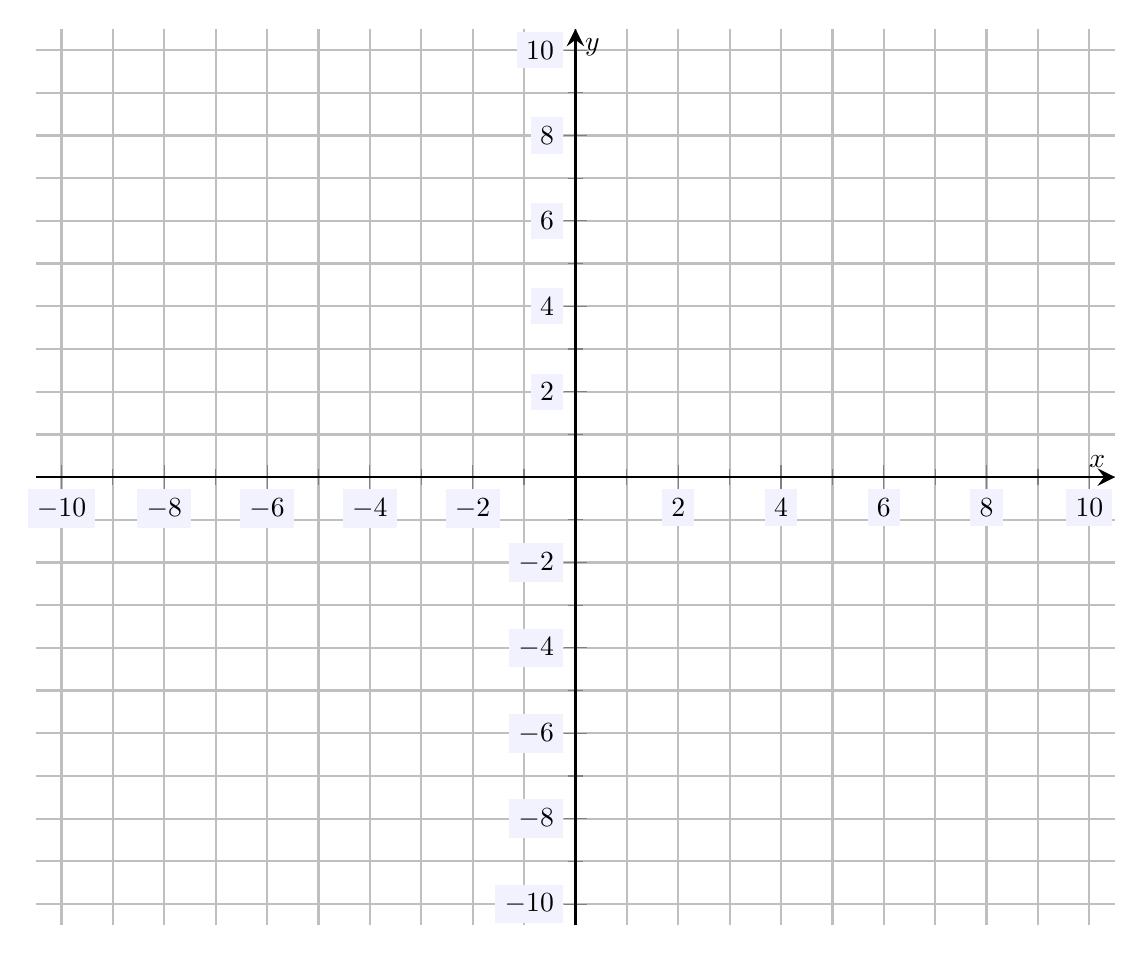
\begin{tikzpicture}[scale=2,every node/.style={scale=0.5}]
	\begin{axis}[
	grid=both,
	axis lines=middle,
	ticklabel style={fill=blue!5!white},
	xmin= -10.5, xmax=10.5,
	ymin= -10.5, ymax=10.5,
	xtick={-10,-8,-6,-4,-2,0,2,4,6,8,10},
	ytick={-10,-8,-6,-4,-2,0,2,4,6,8,10},
	minor tick = {-10,-9,...,10},
	xlabel=\(x\),ylabel=\(y\),
	]
	\end{axis}
	\end{tikzpicture}
	}
	\] 



% Question 2
\newpage
\question[10] Showing all your work, write the exponential function below in the form $y= Ab^x$.
	\[
	-3 \left( \dfrac{2}{7} \right)^{2x - 1}
	\]



% Question 3
\newpage
\question[10] Fully justifying your answer, determine whether each of the following functions exhibit exponential growth or exponential decay:
	\begin{enumerate}[(a)]
	\item $-7 \left( \dfrac{12}{11} \right)^x$
	\item $5 \left( \dfrac{2}{3} \right)^{-x}$
	\item $4 (2^{1 - x})$
	\end{enumerate}



% Question 4
\newpage
\question[10] Showing all your work, rewrite each of the following exponential equations as a logarithmic equation or logarithmic equation as an exponential equation:
	\begin{enumerate}[(a)]
	\item $\log_4(x)= y$
	\item $e^{3y}= x$
	\item $\log_x(5)= y$
	\end{enumerate}



% Question 5
\newpage
\question[10] Showing all your work, compute each of the following:
	\begin{enumerate}[(a)]
	\item $\log_3(81)$
	\item $\ln(1)$
	\item $\log_5(5^{6741})$
	\item $\ln(\sqrt[3]{e^2})$
	\item $\log_{1/2} \left( \dfrac{1}{\sqrt{2}} \right)$
	\end{enumerate}



% Question 6
\newpage
\question[10] Showing all your work, write the following as a single logarithm:
	\[
	\dfrac{1}{3}\, \big( 6 \ln(x) - 2 \ln(y) + \ln(z) \big)
	\]



% Question 7
\newpage
\question[10] Assume $\log_4(x)= -3$, $\log_4(y)= 5$, and $\log_4(z)= -2$. Showing all your work, compute the following:
	\[
	\log_4 \left( \dfrac{x^3 \sqrt{y}}{z^5} \right)
	\]



% Question 8
\newpage
\question[10] Showing all your work and simplifying as much as possible, express the following as a single logarithm in base 2:
	\[
	\log_2(x) - \log_4(x) + \log_8(x)
	\]



% Question 9
\newpage
\question[10] Showing all your work, determine how many digits are in $1728^{1729}$ when expressed in base 10. 



% Question 10
\newpage
\question[10] Showing all your work, determine how many digits are in $1728^{1729}$ when expressed in base 2. 



% Question 11
\newpage
\question[10] Showing all your work, determine if there is an integer $k$ such that $3^k$ has 2022 digits when expressed in base 10. If there is such an integer, find them all. If not, explain why. 



% Question 12
\newpage
\question[10] Gerald meets with the banker Vivildi and decides to invest \$212 with him. Vivildi promises a return of 2.7\% annual interest, compounded quarterly. How much interest will Gerald have earned after 3~years?



% Question 13
\newpage
\question[10] Filipa takes out a loan of \$1000 at 9.4\% annual interest, compounded continuously. How long until Filipa's amount owed has doubled?



% Question 14
\newpage
\question[10] Cirri deposts \$162 in an account which earns 6.6\% annual interest, compounded monthly. How long until Cirri's account has \$4000?



% Question 15
\newpage
\question[10] Showing all your work, solve the following equation:
	\[
	15 - 4(3^{1-x})= 10
	\]



% Question 16
\newpage
\question[10] Showing all your work, solve the following equation:
	\[
	3 \big( \log_7(2x + 1) - 4 \big)= 12
	\]



% Question 17
\newpage
\question[10] Showing all your work, solve the following equation:
	\[
	4 e^{x^2} + 20= 54
	\]



% Question 18
\newpage
\question[10] Showing all your work, solve the following equation:
	\[
	\log_2(3 - x) - 1= 1 - \log_2(x + 3)
	\]



% Question 19
\newpage
\question[10] Showing all your work, solve the following equation:
	\[
	2 (7^{6 - x}) + 4= 24
	\]



% Question 20
\newpage
\question[10] Showing all your work, solve the following equation:
	\[
	\log_2(x - 2)= 2 + \log_2 \left( \dfrac{1}{x + 1} \right)
	\]


\end{questions}
\end{document}